\section{Koncepcja proponowanego rozwiązania}

\qquad Algorytm klasyfikacji załamków QRS został podzielony na trzy części. Najpierw dane wejściowe zostają znormalizowane i zkwantyzowane, następnie przeprowadzana jest procedura ekstrakcji cech. W drugiej części następuje klasyfikacja zespołów QRS. Polega on na  klasteryzacji danych, czyli grupowaniu ich w klasy, które mają najwięcej wspólnych cech. Warto zaznaczyć, iż każdy współczynnik reprezentuje inną wielkość i z tego powodu wartość tolerancji jest dobierana dla każdego z nich indywidualnie. Do klasteryzacji wykorzystywany jest algorytm g-means clustering. Jego realizacją zajmują się klasy GMeans i SVMClassifier.

\subsection{Klasteryzacja}

\qquad Do grupowania danych w klastry (lub klasy) użyto algorytmu G-średnich (ang. "G-means"). Jest rozszerzeniem popularnego algorytmu k-średnich, który polega na dobraniu $k$ klas w zbiorze danych tak, aby dla każdego punktu był on w klasie, do której środka ciężkości ma najbliżej \cite{KMeans}. Przyjęto, że dane, które należy pogrupować to $d$-wymiarowe wektory należące do zbioru $X$ o liczności $n$. $S$ to zbiór klas, a więc $S_{j} = \{x_{i} \in X | klasa(x_{i}) = j\}$ dla $i = 1, 2, ..., n$. Zbiór środków ciężkości klas oznaczony został literą $C$ i zdefiniowany jako: $C = \{c_{j} = \frac{\sum_{x \in S_{j}} x}{|S_{j}|}\}$ dla $j = 1, 2, ..., k$.
Cel algorytmu k-średnich to minimalizacja wyrażenia przedstawionego wzorem \ref{eq:kmeans} .
\begin{equation}
\label{eq:kmeans}
\sum_{j=1}^{k}\sum_{x \in S_{j}} \|x - c_{j}\|
\end{equation}

Poważnym problemem tego algorytmu jest fakt, iż liczba klas musi być znana bądź przyjęta z góry, co oznacza jakąś wcześniejszą wiedzę na temat klasteryzowanego zbioru danych \cite{GMeans, GMeansExplanation}. W przypadku, gdy takiej wiedzy się nie posiada, należy zastosować uogólnienie algorytmu k-średnich, które pozwoli dobrać optymalne $k$ względem pewnego wskaźnika jakości.
Algorytm, który został zastosowany w opisywanym module dobiera $k$ tak, aby w każdej klasie rozkład punktów był możliwie bliski rozkładu normalnego. Stąd też wzięła się litera "G" w nazwie - od rozkładu Gaussa \cite{GMeans}.

Metoda G-średnich zaczyna od niewielkiej liczby klas, by później odpowiednio zwiększać $k$ - nie jest przewidziana procedura zmniejszania tego parametru. W pierwszym kroku zwykle przyjmowane jest $k = 1$, z czego wynika, że $C$ jest zbiorem jednoelementowym, zawierającym środek ciężkości całego zbioru $X$ \cite{GMeans}. W każdym kroku algorytm sprawdza, czy dana klasa ma rozkład normalny, a jeśli nie, to dodaje jej dodatkowy środek. Między każdym takim dodawaniem środków jest używana procedura k-średnich, aby poprawić jakość rozwiązania.

Sprawdzenie normalności rozkładu wewnątrz klasy odbywa się za pomocą testu Andersona - Darlinga. 

\subsection{Klasyfikacja}

\qquad Aby sklasyfikować powstałe w poprzednim kroku klastry wykorzystano klasyfikator SVM (Support Vector Machine). W najprostszej postaci klasyfikator ten służy do wyznaczenia hiperpłaszczyzny rozdzielającej dwa liniowo separowalne zbiory. Hiperpłaszczyzna ta wyznaczana jest z maksymalnym marginesem, tzn. tak, aby suma jej odległości od najbliższych próbek z obu klas była jak największa (patrz rys. \ref{fig:SVM}).

\begin{figure}[h]
	\centering
	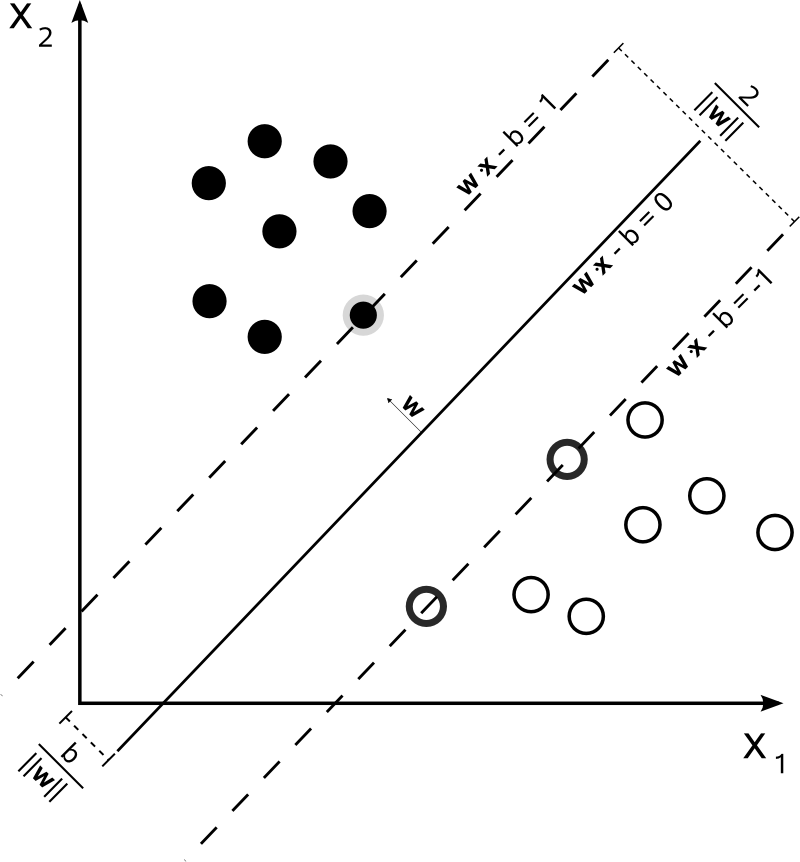
\includegraphics[width=8cm]{Grafika/Svm_max_sep_hyperplane_with_margin}
	\caption{Dwuwymiarowy przypadek hiperpłaszczyzny rozdzielającej dwie klasy z zaznaczonym marginesem. Źródło \cite{SVMWiki}}
	\label{fig:SVM}
\end{figure}

\qquad W wielu przypadkach nie można zagwarantować liniowej separowalności zbiorów.  W takich sytuacjach stosuje się tzw. Kernel trick. Polega on na zwiększeniu wymiaru przestrzeni danych wejściowych, aby w nowej przestrzeni istniała własność liniowej separowalności zbiorów. W tym celu wykorzystuje się różne funkcje jądra (kernel functions). W opisywanym module wykorzystana została funkcja RBF (Radial Basis Function) określona wzorem:

\begin{equation}
\label{eq:RBF}
K(x,x') = \exp{\left(-\frac{{\|x-x'\|}^{2}}{2\sigma^2}\right)}
\end{equation}

\qquad Aby klasyfikator mógł działać wcześniej należy go wytrenować. Polega to na podaniu mu ciągu wektorów uczących. Opisywany klasyfikator został wytrenowany za pomocą bazy danych MIT-BIH Arrhythmia Database \cite{MITDB}. Gotowy model klasyfikatora wczytywany jest z pliku, w którym zapisane są różne parametry oraz zestaw wektorów nośnych, na których opiera się działanie metody SVM.
